\documentclass[11pt,a4paper]{article}
\usepackage[margin=2.2cm]{geometry}
\usepackage{fontspec}
\setmainfont{TeX Gyre Pagella}
\setmonofont{DejaVu Sans Mono}[Scale=0.82]
\usepackage{amsmath,amssymb,amsthm}
\usepackage{graphicx,xcolor,listings,booktabs,enumitem}
\usepackage[most]{tcolorbox}
\usepackage{tikz}
\usepackage{needspace}
\usepackage[hidelinks]{hyperref}

\definecolor{accent}{HTML}{2B6CB0}
\definecolor{warn}{HTML}{C53030}
\newtcolorbox{keybox}[1][]{colback=accent!5,colframe=accent,boxrule=0.6pt,arc=2pt,left=6pt,right=6pt,top=4pt,bottom=4pt,#1}
\newtcolorbox{warnbox}{colback=warn!5,colframe=warn,boxrule=0.6pt,arc=2pt,left=6pt,right=6pt}

\lstdefinelanguage{Rust}{
  keywords={fn,let,mut,if,else,for,in,while,return,use,pub,struct,impl,loop,break,Some,None,as,match,const,Self,self},
  morekeywords=[2]{usize,i32,i64,u64,f64,bool,Vec,VecDeque,BTreeSet,BTreeMap,BinaryHeap,Option,str},
  sensitive=true, morecomment=[l]{//}, morestring=[b]"}
\lstset{language=Rust,basicstyle=\ttfamily,keywordstyle=\color{accent}\bfseries,
  keywordstyle=[2]\color{teal},commentstyle=\color{gray}\itshape,stringstyle=\color{warn},
  frame=single,rulecolor=\color{gray!40},backgroundcolor=\color{gray!4},
  numbers=left,numberstyle=\tiny\color{gray},xleftmargin=1.5em,breaklines=true,
  columns=fullflexible,keepspaces=true,showstringspaces=false}

\newtheorem*{invariant}{Invariant}
\theoremstyle{definition}\newtheorem*{definition}{Definition}

\usepackage{soul}
\definecolor{hlY}{HTML}{FFF3A0}\definecolor{hlG}{HTML}{C8F2C2}\definecolor{hlP}{HTML}{E6D2F7}\definecolor{hlB}{HTML}{CFE3FF}
\newcommand{\hly}[1]{{\sethlcolor{hlY}\hl{#1}}}
\newcommand{\hlg}[1]{{\sethlcolor{hlG}\hl{#1}}}
\newcommand{\hlp}[1]{{\sethlcolor{hlP}\hl{#1}}}
\newcommand{\hlb}[1]{{\sethlcolor{hlB}\hl{#1}}}
\newcommand{\img}[3]{\begin{center}\begin{minipage}{\linewidth}\centering\fcolorbox{gray!50}{white}{\includegraphics[width=#1]{board/#2}}\\[-2pt]{\footnotesize\textcolor{gray}{#3}}\end{minipage}\end{center}}
\newcommand{\extra}{\textsuperscript{\textcolor{warn}{[extra]}}}
% pages of the prof's 2025 notes on the segment tree (Lessons/L13/Segment_tree_2025.pdf)
\newcommand{\stnote}[2]{\begin{center}\fcolorbox{gray!50}{white}{\includegraphics[page=#1,width=#2,trim=20 20 20 20,clip]{../L13/Segment_tree_2025.pdf}}\\[-2pt]
  {\footnotesize\textcolor{gray}{Prof.'s notes of \textbf{last year} (2025), \texttt{Segment\_tree\_2025.pdf} p.\,#1}}\end{center}}
\newcommand{\stnotes}[2]{\begin{center}\begin{minipage}{0.49\textwidth}\centering\fcolorbox{gray!50}{white}{\includegraphics[page=#1,width=0.95\linewidth,trim=20 20 20 20,clip]{../L13/Segment_tree_2025.pdf}}\end{minipage}\hfill
  \begin{minipage}{0.49\textwidth}\centering\fcolorbox{gray!50}{white}{\includegraphics[page=#2,width=0.95\linewidth,trim=20 20 20 20,clip]{../L13/Segment_tree_2025.pdf}}\end{minipage}\\[2pt]
  {\footnotesize\textcolor{gray}{Prof.'s notes of \textbf{last year} (2025), \texttt{Segment\_tree\_2025.pdf} p.\,#1 and p.\,#2}}\end{center}}
\newcommand{\yn}{\textsuperscript{\textcolor{accent}{[your notes]}}}
\newcommand{\notyn}{\textsuperscript{\textcolor{warn}{[not in your notes]}}}
\newcommand{\pfig}[3]{\begin{center}\begin{minipage}{\linewidth}\centering\includegraphics[width=#1]{figs_prof/#2.pdf}\\[-1pt]
  {\footnotesize\textcolor{gray}{Prof.'s 2026 notes (\emph{Segment Tree}, blog): #3}}\end{minipage}\end{center}}
\newcommand{\board}[3]{\img{#1}{#2}{Board, #3 (recording \texttt{L\_14.MP4})}}
\title{\textbf{CPC --- Lecture 14}\\[2pt]\large Segment tree: cost of \textsf{RangeSum} $\cdot$ dynamic RMQ $\cdot$ RMQ with occurrences $\cdot$ \textsf{Search} $\cdot$ \#occs (statement)}
\author{Competitive Programming and Contests --- Monday 02/11/2026}
\date{}

\begin{document}\sloppy
\maketitle
\vspace{-1.5em}
\begin{keybox}
\textbf{Sources.} Recording \texttt{Lessons/L14/L\_14.MP4} (90 min) and its automatic transcript \texttt{L14\_transcript.txt} (not revised);
the prof's handwritten board (frames of the recording, \texttt{board/l14\_*.jpg}); your notes taken in class (\texttt{Lessons/L14/notes.md}, marked \yn{} where quoted);
the prof's 2025 notes \texttt{Lessons/L13/Segment\_tree\_2025.pdf} p.\,3--9 (always marked \emph{last year}); course page (checked 11/11/2026); \textbf{the prof's 2026 notes} \emph{Segment Tree} (blog, published 14/11/2026, \S\ref{sec:blog}).
The prof has no blog post on segment trees. Everything marked \extra{} was \emph{not} said or written in the lecture.

\smallskip
\noindent Code: \texttt{Lessons/L14/src} (\texttt{cargo test -p l14}): \texttt{prof\_blog} = the prof's code from the 2026 notes (verbatim); the rest is mine \extra. Exercises: \texttt{Lessons/L14/practice}, E56--E58 (\texttt{cargo test -p practice\_l14}).

\smallskip
\noindent\textbf{Highlights:} \hly{general / to remember} \quad \hlg{good: works, efficient, correct} \quad \hlp{bad: pitfalls, wrong ideas, costs} \quad \hlb{definitions and key results}
\end{keybox}

\begin{keybox}[colback=gray!4,colframe=gray!60]
\textbf{Where we are.} L13 (28/10) introduced the segment tree for dynamic prefix sums and ended with the question \emph{``is \textsf{RangeSum} linear, or better?''}.
Today: recap of the segment tree and of the \textsf{RangeSum} visit (0:00--14:00), \textbf{the answer: $O(\log n)$ nodes} (14:00--49:00),
then \hly{the same recipe applied to other problems}: \textbf{dynamic RMQ} (50:00--60:00), \textbf{RMQ with occurrences} (60:00--69:00),
\textbf{\textsf{Search}$(s)$} (70:00--87:40), and the \textbf{statement of \#occs} (88:00--90:00), left to think about.
\hlp{Next week (09/11 and 11/11) there is no lecture}: the prof is at a conference (``See you on Wednesday. Next week, no lecture'').
\end{keybox}

\tableofcontents

%==========================================================
\section{Recap: the segment tree and the golden rule}
%==========================================================
The idea (0:00--2:10): \hly{group consecutive elements of the array} in pairs, pairs of pairs, and so on: a (perfect, if $n$ is a power of 2) binary tree on top of the array.
Then the approach that segment trees always follow, the \hlb{golden rule}: \hlb{for every node, store the answer of the query for the node's range}.
\hly{The structure of the tree is fixed and depends only on $n$; what goes in the nodes depends on the query}: here the sums, the root holds the sum of the whole array.
\begin{itemize}[nosep]
\item \textsf{Add}$(i,v)$: change the leaf and \hlg{go up to the root} updating the nodes on the path: \hlb{\mbox{$\Theta(\log n)$}}, the height of the tree (board: $\textsf{Add}(4,+3)$).
\item \textsf{RangeSum}$(i,j)$: from the root, compare the node's range with the query range (``rescaled'' to the part that falls in the subtree, e.g.\ $[2,5]$ becomes $[2,3]$ on the left and $[4,5]$ on the right):
  \hlb{no overlap} $\to$ stop, nothing to return; \hlb{total overlap} $\to$ stop and return the node's value; \hlb{partial overlap} $\to$ recurse \emph{both} left and right and \hly{combine} the results (here: sum).
\end{itemize}
\board{0.62\textwidth}{l14_rs_visit.jpg}{13:40: $\textsf{RS}(2,5)$ on $A=[3,1,-2,4,6,13,2,0]$; po/to/no = partial/total/no overlap; result $2+19=21$}
\noindent\extra{} Test \texttt{range\_sum::board\_examples\_2026}: $\textsf{RS}(2,5)=21$ visiting 7 nodes, $\textsf{Add}(4,+3)$ gives 24.

%==========================================================
\section{The cost of \textsf{RangeSum}: $O(\log n)$ nodes}
%==========================================================
\textbf{The worry} (14:00). \hlp{A recursive algorithm that goes both left and right may traverse the whole tree}; in the small example it touches \emph{all} the internal nodes.
Is the algorithm inefficient, or is the example too small? With $n=8$ we cannot see the difference between ``something like $8\log n$'' and $n$: the constant in front of $\log n$ hides it.
A student: \hlg{doubling $n$ adds a level, but the algorithm would prune many more nodes}. Another student: one can check the children before recursing (``anticipate the no overlap''):
\hly{this only moves the work} (you still check each child), it saves one recursive step, not the work.

\noindent\textbf{The right question} (20:00): \hlb{how many nodes do we process?} It is more general than ``what is the running time'':
\hly{time = number of touched nodes $\times$ cost of processing one node}. For sums each node costs $O(1)$, but \hly{there are segment-tree problems where processing a node is not constant time}.

\board{0.6\textwidth}{l14_overlap_cases.jpg}{26:00: the three kinds of overlap, and the three kinds of partial overlap (dashed line = middle of the node)}
\noindent\textbf{Case analysis} (21:40--30:00).
\begin{itemize}[nosep]
\item No overlap and total overlap are the \hlg{easy cases}: the recursion stops there.
\item \hlp{Partial overlap is the problematic case}, because it always goes both left and right. It has three sub-cases (dashed line = the node's middle):
  the query is \textbf{entirely left} of the middle, \textbf{entirely right}, or \textbf{split by the middle}.
\item Left/right: \hlg{easy cases, because one of the two branches stops immediately} (no overlap). If there were only these, we would follow a single path: logarithmic.
\end{itemize}
\board{0.4\textwidth}{l14_easy_cases.jpg}{29:00}
\noindent\textbf{The only hard case} (30:00--38:50): the middle splits the query. Both children get a partial overlap... but \hlb{special ones}:
since the split point lies inside the query, \hlb{the left child's query part ends exactly at the child's right extreme, and the right child's part starts exactly at its left extreme}.
With one extreme fixed, only the length can change, so in each of these ``special'' nodes, of the two grandchildren \hlg{one is a total overlap or a no overlap} (the easy one),
and only the other one keeps going --- again with the same extreme fixed.
\board{0.62\textwidth}{l14_special_pos.jpg}{46:20: ``special po'' and the shape of the visit}
\noindent\textbf{Shape of the visit} (39:00--45:00): \hlb{one path from the root to the first node that splits the query}, then \hlb{two paths} (one per side) down to where the recursion stops,
and along each path every node has one ``easy'' sibling that stops immediately. Splitting happens \hly{just once in the whole search}.
\begin{itemize}[nosep]
\item Worst case: the split node is the root and both paths reach the leaves: $2\log n$ path nodes, plus one easy sibling each: \hlb{\mbox{$4\log n$} touched nodes}.
\item With the student's trick (never enter a child if not needed): $2\log n$ nodes, \hlp{saving a factor 2 in nodes but not in work}, since you still have to check.
\item Prof's example of a long visit with a tiny query (46:00): \hly{two adjacent elements just around the root's middle}: the shortest query with more than one element, but two full root-to-leaf paths.
\end{itemize}
\hlb{So every query touches $O(\log n)$ nodes; with $O(1)$ per node, \textsf{RangeSum} is \mbox{$\Theta(\log n)$}, not linear.}
Recap (47:50--49:40): tree on top of the array, golden rule, update leaf$\to$root, query root$\to$down with the three cases,
\hly{the node combines the answers of its children}, \hlg{build bottom-up in linear time}, \hlg{both operations logarithmic}.
\stnotes{3}{4}
\noindent\extra{} Brute-force check over all ranges (\texttt{l14::range\_sum}, test \texttt{visited\_nodes\_at\_most\_4\_per\_level}; prof's adjacent-pair case in \texttt{board\_examples\_2026}: 39 nodes for $n=1024$, i.e.\ $1+2+4\cdot 9$):
\begin{center}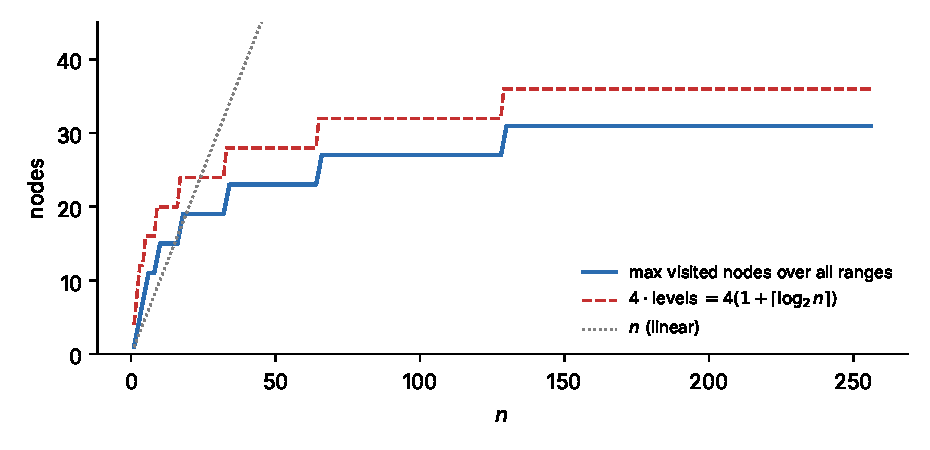
\includegraphics[width=0.72\textwidth]{figs/l14_visited.pdf}\\[-2pt]{\footnotesize\textcolor{gray}{\extra{} Maximum number of visited nodes over all ranges, tree split in the middle.}}\end{center}

%==========================================================
\section{Dynamic Range Minimum Queries}
%==========================================================
\hly{From now on: we know the structure and the idea; we solve problems by applying the approach.} \hlg{Easy problems} first (50:00).

\noindent\textbf{Problem.} \textsf{Add}$(i,v)$ and \hlb{\mbox{$\textsf{RMQ}(i,j)=\arg\min A[i..j]$}, the \emph{position} of the minimum in $A[i..j]$}.
``It seems an exotic query, but it is very, very useful in practice, for many problems.''

\noindent\textbf{Solution.} Same tree; by the golden rule \hlb{every node stores the minimum of its range}.
To return the position, store the pair (min, position), or \hly{just the position and use it to access $A$} (a student, 63:00); the prof writes the minimum values on the board
``because it is easier for us humans'', but most applications use the arg min.
\board{0.48\textwidth}{l14_rmq_tree.jpg}{56:00: the minima; the query $[2,5]$ is split into $[2,3]$ and $[4,5]$}
\begin{itemize}[nosep]
\item \textsf{RMQ}: \hlg{exactly the same visit}; the results of the total-overlap nodes are combined with $\min$: on $[2,5]$, $\min(-2,6)=-2$.
\item \hlb{The visit splits the query range into sub-intervals}: from 1 up to $O(\log n)$ of them (not $n$, or the algorithm could not be logarithmic), and \hlb{they never overlap}
      (a node with total overlap stops the recursion, so nothing below it is reached).
      \hly{For the sum non-overlapping is crucial (otherwise double counting); for the min it is not}: the min is correct even with overlaps. ``This is going to be useful when we discuss other solutions for RMQ.''
\item \textsf{Add}$(2,+7)$: $-2\to5$; node $[2,3]$: $\min(5,4)=4$; $[0,3]$: $\min(1,4)=1$; root: $\min(1,0)=0$.
      \hly{At every node: the new min of one child, the old min of the other, take the min}: $\Theta(\log n)$.
      Early stopping (as soon as the changed position is no longer the parent's minimum nothing changes above) \hlp{is a heuristic: it does not improve the worst case}.
\end{itemize}
\board{0.5\textwidth}{l14_rmq_add.jpg}{60:00: $\textsf{Add}(2,7)$}
\noindent Your notes: ``with the prev.\ ex.\ we reach $-2$ and $6$ for query $[3,6]$'' \yn: the query on the board was $[2,5]$ (nodes $[2,3]$ and $[4,5]$).
\extra{} \texttt{l14::rmq::RmqTree} (ties: leftmost position), test \texttt{board\_example\_2026} and against a linear scan.

%==========================================================
\section{Range Minimum Queries with occurrences}
%==========================================================
\textbf{Problem} (60:20). \textsf{Add}$(i,v)$ and \hlb{\mbox{$\textsf{query}(i,j)$}: the minimum value in $A[i..j]$ with its number of occurrences in $A[i..j]$}.
A student: \hlg{store also a counter}. Golden rule again: the problem asks for (min, \#occurrences), so \hlb{every node stores the pair (value, \#occs) for its range}.

\noindent\textbf{Why it works.} The query splits the range into sub-intervals; each returns its own (min, count). \hlb{Sum the counts of the sub-intervals whose min equals the overall minimum};
a sub-interval with a different (so larger) min does not contain the overall minimum at all, and its count is discarded.
Example $A=[3,0,0,4,0,13,2,0]$: root $(0,4)$; $\textsf{query}(2,5)$: $(0,1)$ and $(0,1)$ $\to$ $(0,2)$.
After $\textsf{Add}(4,13)$ ($0\to13$): $[4,5]=(13,2)$, $[4,7]=(0,1)$, root $(0,3)$; now $\textsf{query}(2,5)$ combines $(0,1)$ and $(13,2)$ $\to$ \hlb{$(0,1)$, not $(0,2)$}.
Updates touch only the $\log n$ nodes on the path.
\board{0.55\textwidth}{l14_rmq_occ_add.jpg}{69:20: (value, \#occs) in every node, then $\textsf{Add}(4,13)$}
\noindent The prof's comment (68:30): for easy problems the approach is ``almost trivial'': draw the tree and put the answer in each node.
\hlp{A segment tree uses more space than a Fenwick tree}, but \hlg{it is much more general}; for harder problems the recipe is the same, \hlp{but storing the answer may be much more complicated}.
\stnotes{5}{6}
\noindent\extra{} \texttt{l14::rmq\_occ::MinCountTree}, test \texttt{board\_example\_2026} (this example) and \texttt{example\_2025\_notes} (last year's: $A[7]\colon 0\to-2$).

%==========================================================
\section{\textsf{Search}$(s)$: smallest $i$ with prefix sum $\ge s$}
%==========================================================
\textbf{Problem} (70:00). $A[1,n]$ of \hlp{non-negative} integers (positions from 0 on the board); \textsf{Add}$(i,v)$, \textsf{RangeSum}$(i,j)$ and
\hlb{\mbox{$\textsf{Search}(s)$}: the smallest position $i$ such that \mbox{$\sum_{k=0}^{i}A[k]\ge s$}} (the board first says ``the position of the shortest prefix of $A$'', then rewrites it this way).
\hly{Non-negative values: the prefix sums never decrease}, so from the answer on they are always $\ge s$.
\board{0.5\textwidth}{l14_search_statement.jpg}{74:40: $A=[3,1,0,4,6,13,2,0]$, prefix sums $3,4,4,8,14,27,29,29$: $\textsf{Search}(22)=5$}
\noindent The tree of the previous problems cannot be used as it is: it has $-2$ (\hlp{negative}); the prof changes it to $0$ (root 29).

\noindent\textbf{Specialized solution} (77:20--83:30, suggested by a student). Start from the root; \hly{compare $s$ with the left child's sum}:
if it is enough, the answer is in the left half; otherwise go right searching for \hly{$s$ minus the left sum} (``we subtract something only when we go right'').
Board: 22 vs 8 $\to$ right with $22-8=14$; at $[4,7]$: 14 vs 19 $\to$ left (search 14); leaf 6 $<14$ $\to$ right with $14-6=8$; leaf 13 $\ge 8$ $\to$ \textbf{position 5}.
At a leaf two cases: its value is greater than what we are looking for, or equal (the prefix sum is exactly $s$); either way that is the answer.
\board{0.55\textwidth}{l14_search_visit.jpg}{86:00: $\textsf{Search}(22)$}
\noindent Cost: we may go left and then come back and go right, but \hlg{when we go both ways the left step was cheap (one step)}: \hlb{\mbox{$\Theta(\log n)$}}.
(The transcript around 79:00--80:30 is a bit confused about which node is compared with what; the board and the result are clear.)

\noindent\textbf{The checklist} (83:30--87:40). \hly{``Segment tree must go directly in your checklist''} (item ``use standard data structures''). The second item, \hly{binary search for the answer}, also works:
the prefix sums are monotone, so ``is the prefix sum up to $i$ $\ge s$?'' is a valid predicate; $\log n$ steps, each one a prefix sum in $\log n$: \hlp{\mbox{$\Theta(\log^2 n)$}, a log factor more}.
It is \hlp{particularly inefficient}: every step restarts from the root and recomputes the same nodes, while the specialized solution sees immediately from a node which side to take.
\hly{The checklist gives you some help, but not always the final solution: look at the problem and find more appropriate solutions.}
(Your notes: ``but less space'' for the binary search version \yn{} --- not in the transcript.)
\stnotes{7}{8}
\noindent\extra{} \texttt{l14::search::SearchTree::search} ($\Theta(\log n)$) and \texttt{search\_binary} ($\Theta(\log^2 n)$), both against a linear scan.

%==========================================================
\section{\#occs: occurrences of $x$ in a range (statement only)}
%==========================================================
\textbf{Problem} (88:00). $A[0,n-1]$ of integers; \textsf{Add}$(i,v)$ and \hlb{\mbox{$\#\textsf{occs}(i,j,x)$}: the number of occurrences of $x$ in $A[i..j]$}.
Reporting the occurrences of the \emph{minimum} is what we already saw; \hly{what about an arbitrary $x$?}
\board{0.55\textwidth}{l14_occs_statement.jpg}{90:20}
\begin{warnbox}
\textbf{Homework (spoken).} ``You may try to find the solution if you have time.'' Next lecture: \hly{we conclude the segment tree presenting many other problems}, starting from this one,
where \hlp{storing a number in each node is no longer enough: you need to store more}.
The solution is in \texttt{Lessons/L15/L15.pdf} (from the prof's 2026 notes) and in last year's notes (p.\,9): try before looking.
\end{warnbox}
\noindent\extra{} \texttt{l14::occs::OccsTree} implements last year's solution (hash map per node).

%==========================================================
\section{The prof's 2026 notes on this lecture}\label{sec:blog}
%==========================================================
On 14/11 the prof published \emph{Segment Tree} (\url{https://pages.di.unipi.it/rossano/blog/2026/segmenttree/}), written ``with the help of a trusted friend'' (an AI):
it covers L13--L15 in one text, with a different running example, $A=[5,1,3,1,4,7,2,1]$. The parts of this lecture are:
\emph{How many nodes do we visit?} (the analysis of \S2), \emph{Segment Tree in Rust}, \emph{Beyond Sums}, \emph{Dynamic Range Minimum Queries},
\emph{Minimum with Number of Occurrences}, \emph{Searching on a Segment Tree}. Same content as the lecture; the useful differences:
\begin{itemize}[nosep]
\item The cost analysis names the three kinds of partial overlap: the query part inside one half; a \hlb{suffix or prefix crossing the middle} (one child total overlap);
      the \hlb{general partial overlap} $l<i\le m<j<r$. Its children get \hlb{anchored} query parts (a suffix of the left child, a prefix of the right child),
      and \hlg{an anchored part can never produce a general partial overlap}: so \hlb{at most one general partial overlap}, then two paths, at most 4 nodes per level.
      (This is the ``special po'' of the board.)
\item Code: root = node 0, children $2u+1$, $2u+2$ (heap layout), vector of $4n$ nodes. \hly{Why $4n$}: indexes are not contiguous when $n$ is not a power of 2
      (for $n=6$ the leaf 4 is node 12); height $h=\lceil\log n\rceil$, indexes $<2^{h+1}$ and $2^h<2n$.
\item \textsf{Search} returns \texttt{None} if the root does not reach $s$: \hlp{without this check the descent ends in the last leaf} and returns a wrong answer.
\item The checklist remark of the lecture is not in the notes; \emph{Beyond Sums} (associativity, neutral element, Fenwick vs segment tree) is summarized at the beginning of L15.pdf.
\end{itemize}
\pfig{0.62\textwidth}{st_po_anchor}{the children of a general partial overlap get anchored query parts}
\pfig{0.62\textwidth}{st_complexity}{query $[3,12]$ with $n=16$: one general partial overlap (the root), then two paths}
\pfig{0.5\textwidth}{st_search}{$\textsf{search}(20)$ on the running example: answer 5}
\noindent\extra{} \texttt{l14::prof\_blog::SegmentTree} (the prof's code, verbatim), tested on every number of the notes, on the board examples of L13/L14 and against a naive array;
\texttt{l14::rmq}, \texttt{rmq\_occ}, \texttt{search} also tested on the notes' examples ($\textsf{rmq}(2,7)=3$; root $(1,3)$, after $\textsf{add}(1,-1)$: $(0,1)$; $\textsf{search}(20)=5$). All the numbers of the notes check out.

%==========================================================
\section{Exercises and deadlines (course page)}\label{sec:ex}
%==========================================================
\begin{keybox}
\textbf{Row of 02/11/2026} (``Segment Trees: Lazy Propagation''; the row is the prof's plan --- lazy propagation was \emph{not} done today):
\begin{itemize}[nosep]
\item \emph{Circular RMQ}, \url{http://codeforces.com/problemset/problem/52/C}: \textbf{optional} (not bold) in the row of 02/11/2026.
\end{itemize}
\smallskip
\textbf{Still open, from earlier rows of this year's table} (2026):
\begin{itemize}[nosep]
\item \textbf{Update the Array}, \url{http://www.spoj.com/problems/UPDATEIT/}: mandatory in the row of \textbf{19/10/2026} (explained in L13).
\item \textbf{Nested Segments}, \url{http://codeforces.com/problemset/problem/652/D}: mandatory in the row of \textbf{21/10/2026} (explained in L12);
      \emph{solve Nested Segments with segment trees}: optional in the row of 26/10/2026.
\item \emph{Pashmak and Parmida's problem}, \url{http://codeforces.com/problemset/problem/459/D}: optional, row of 21/10/2026.
\item \textbf{Hands-On 2} (row of 04/11/2026), \url{https://pages.di.unipi.it/rossano/blog/2024/handson2}: \hlp{deadline 22/11/2026} (scaffold in \texttt{HandsOn/HO2}).
\end{itemize}
\end{keybox}
\noindent Practice (\extra, not assigned by the prof): \texttt{Lessons/L14/practice} E56 (dynamic RMQ), E57 (min with occurrences), E58 (\textsf{Search}: $\Theta(\log n)$ and $\Theta(\log^2 n)$).

%==========================================================
\section{Next time}
%==========================================================
``See you on Wednesday'' (04/11 = L15): end of the segment tree, ``many other problems'' starting from \#occs. \hlp{No lecture in the week of 09/11.}
The prof also said he would give the hands-on by the end of that week, to work on it while he is away (Hands-On 2 is on the course page, row of 04/11).
\extra{} L15 has no recording: \texttt{Lessons/L15/L15.pdf} is written from the prof's 2026 notes (\#occs, successor, increasing triplets, lazy propagation, persistent segment tree).

\end{document}
